\documentclass{beamer}
\usepackage[utf8]{inputenc}
\usepackage[T1]{fontenc}
\usepackage{fancyvrb}
\title{Supervised Music Taste Analysis}
\date{WASP Supervised Machine Learning}
\author[Agents 47]{The Hitmen --- Agents 47}

\usetheme{wasp}

\graphicspath{{./graphics/}}

\begin{document}

\begin{frame}
  \titlepage
\end{frame}


\begin{frame}
  \frametitle{Choosen Algorithms}
  \begin{itemize}
  \item Random Forest
  \item Gradient Boost
  \end{itemize}
\end{frame}

\begin{frame}
  \frametitle{Random Forest}
  \begin{itemize}
  \item Based on two concepts: (i)\underline{decision trees} and (ii)\underline{bagging}
  \item \textbf{Bagging} $\rightarrow$ averaging between many small (and not so good) estimators
  \item \textbf{Decision Tree} $\rightarrow$ the formalization of a step-by-step decision process in which different yes-or-no questions are asked to the data unitl a decision is taken
  \item \textbf{Random Forest} $\rightarrow$ comprehends the selection of a number of estimators (i.e. of decision trees) and training each of them on a random subset of the dataset (overfitting will happen, decision trees are affected by this)
  \item When evaluating over new data average the outcome of each of the trained estimators
  \end{itemize}
\end{frame}


\begin{frame}
  \frametitle{Gradient Boosting}
  \begin{itemize}
  \item \textbf{Boosting} combines multiple weak learners, usually iteratively, into a single strong one. If the errors in the learners are uncorrelated the learners can be combined using majority voting. Example of learners are AdaBoost, Gradient Boost and XGBoost.

  \item \textbf{Gradient Boosting} can be seen as an optimization problem where we seek to minimize a loss function. New weak learners are fitted to the residuals of the previous learners, thus minimizing the residuals and reducing the loss function.
  \end{itemize}
\end{frame}


\begin{frame}[fragile]
  \frametitle{The Application}

\begin{Verbatim}[fontsize=\footnotesize]
    Music Taste Analyzer

    positional arguments:
    FILE                  The Music Taste classifier training data.
    FILE                  The new songs to test the classifier on.

    -h, --help            show this help message and exit
    -c {dtree,lda,qda,grdboost,knn,svm,nbayes,gaussproc,mlpc,adaboost,nusvm,rdforest},
    The type of classifier to use.
    -s SEED, --seed SEED  The seed to use for splitting the training data.
    -p PERCENT, --percent PERCENT
    Percent of the training/validation splits.
    -r, --random          Perform a randomized search over the hyperparameters.
    -n N_ITERS, --n-iters N_ITERS
    Number of iterations for the randomized search.
\end{Verbatim}

\end{frame}


\begin{frame}
  \frametitle{Randomized Hyperparameter Search}

  \begin{itemize}
  \item Lots of models - tons of parameters - so little time $\ldots$
  \item \texttt{sklearn.model\_selection.RandomizedSearchCV}.
  \end{itemize}

  \note{Don't bother learning the various parameters of so many models, use
    randomness in your favour instead.}

  \note{\texttt{sk-learn} has a built-in implementation of a randomized
    parameter-space searcher, so let us try that to estimate the parameters.}

\end{frame}


\begin{frame}
  \frametitle{Evaluation}

  \begin{itemize}
  \item Save one initial split.
  \item \texttt{sklearn.model\_selection.RandomizedSearchCV}.
  \item Output the model classification precision.
  \end{itemize}

  \note{Create a first, random split among the training data, use this as a final
    validation dataset.}

  \note{Use RandomizedSearchCV to search for hyperparameters. The number of
    iterations to actually use is configurable by the user.}

  \note{RandomizedSearchCV perform cross-validation internally while searching
    the parameter space, so we output that as well as an estimate of the
    classification performance on the initial split.}

\end{frame}



\begin{frame}
  \frametitle{Results}
  \begin{figure}[ht]
    \centering
    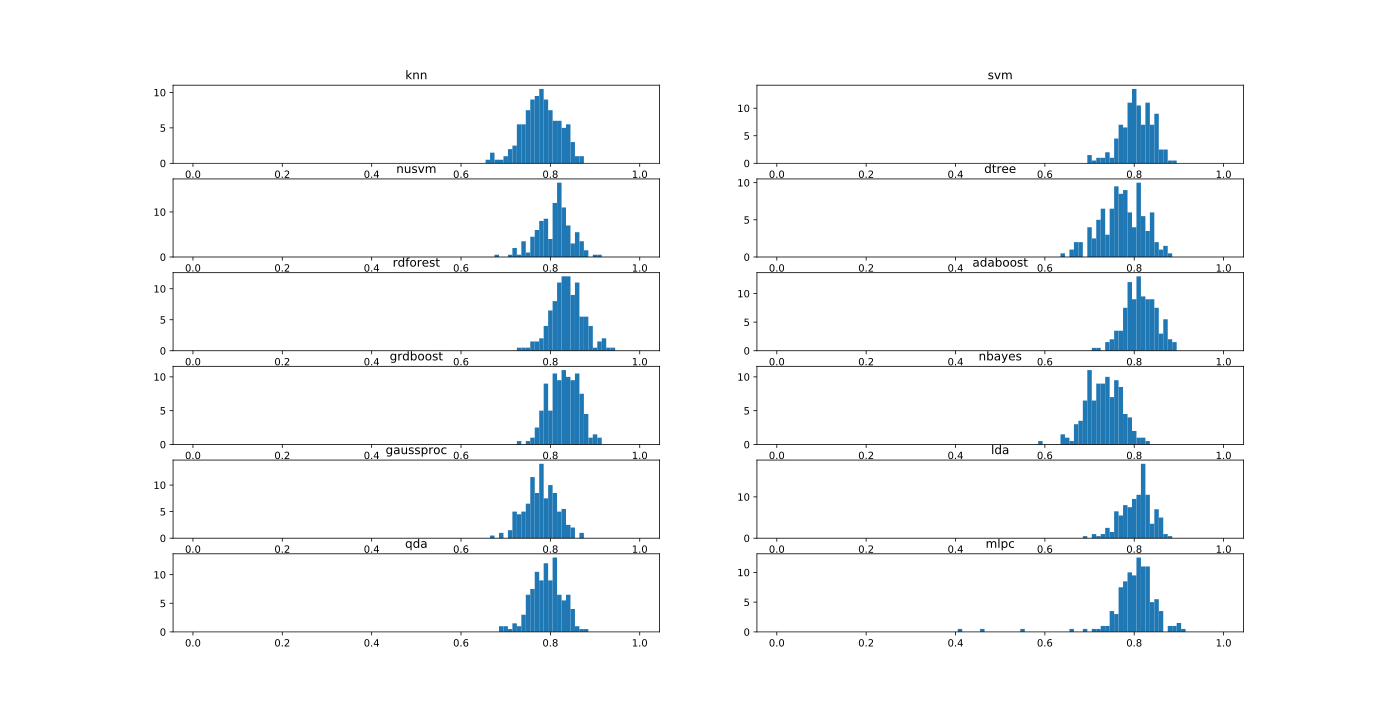
\includegraphics[width=1.0\textwidth]{mc_histograms.pdf}
    \label{fig:mc-histograms}
  \end{figure}
\end{frame}


\begin{frame}
  \frametitle{Results}
  \begin{figure}[ht]
    \centering
    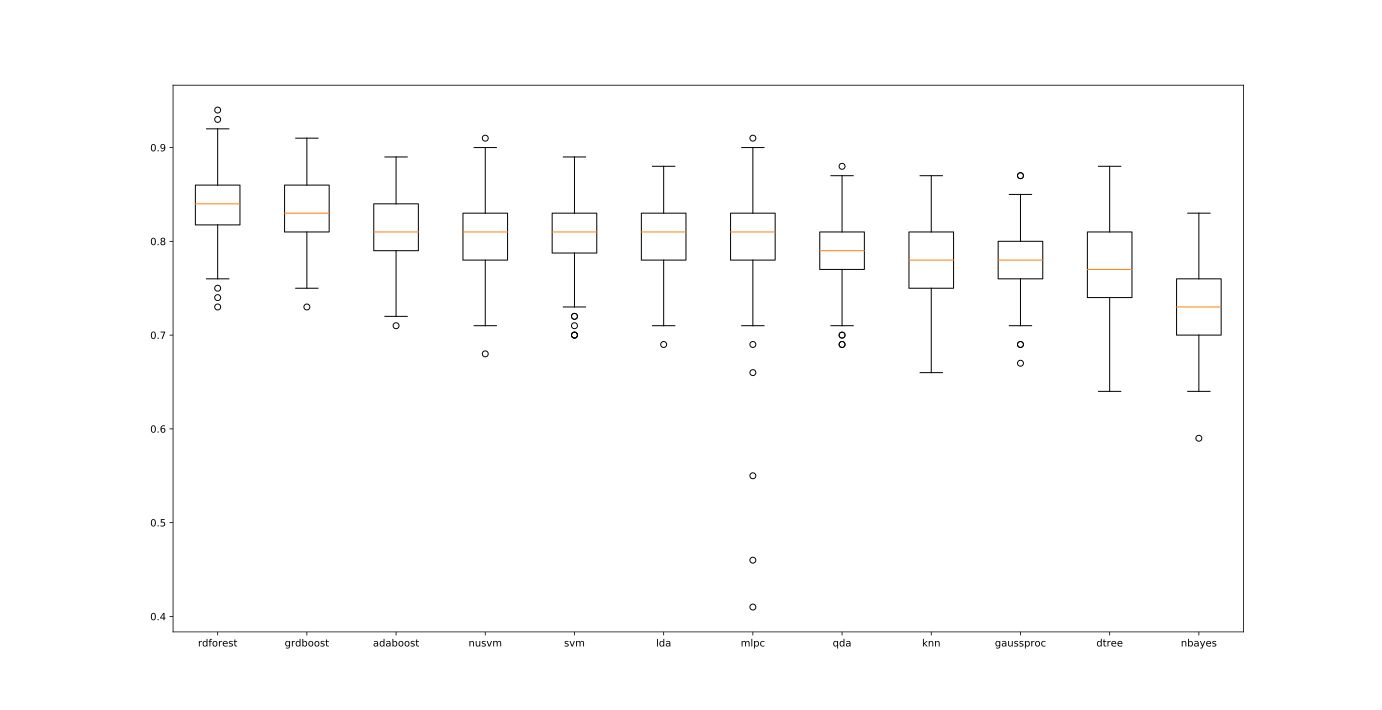
\includegraphics[width=1.0\textwidth]{mc_boxplot.pdf}
    \label{fig:mc-boxplot}
  \end{figure}
\end{frame}


\begin{frame}
  \frametitle{Conclusion and Production Choice}
  \begin{itemize}
  \item 91 \% on test set.
  \item Random Forest performed best, hence our choice.
  \item Relatively simple algorithm to understand.
  \end{itemize}

\end{frame}


\begin{frame}
  \frametitle{Next Steps}

  From here, there are still a number of things one may want to do:

  \begin{itemize}
  \item Apply the model to an actual application?
  \item $\ldots$
  \end{itemize}

\end{frame}

\bgroup
\setbeamertemplate{background}{}
\setbeamercolor{background canvas}{bg=black}
% \setbeamertemplate{navigation symbols}{}
\begin{frame}[t,plain]{}{}
  \begin{center}
    {\tiny \textcolor{white}{The End}}
  \end{center}
\end{frame}
\egroup

\end{document}
